% algorithm.tex -- Algorithms of mpc_cuda
%
% A self-contained description of the algorithms used by mpc_cuda, in the spirit
% of MPFR's "algorithms.tex".  It documents (i) where the runtime cu_mpfr/cu_mpc
% layer departs from upstream MPFR/MPC, and (ii) the compile-time fixed-precision
% register-resident types cu_freal<PB> / cu_fcomplex<PB> and their elementary
% functions, in a form that can be cited from a paper.
%
% Build (no external figure files; pdflatex only):
%     pdflatex algorithm.tex && pdflatex algorithm.tex
%
\documentclass[11pt,a4paper]{article}

\usepackage[T1]{fontenc}
\usepackage{lmodern}
\usepackage{amsmath,amssymb}
\usepackage{booktabs}
\usepackage{array}
\usepackage{microtype}
\usepackage[margin=25mm]{geometry}
\usepackage{tikz}
\usetikzlibrary{positioning,calc,arrows.meta,fit,backgrounds,decorations.pathreplacing,decorations.pathmorphing}
\usepackage{algorithm}
\usepackage{algpseudocode}
\usepackage[hidelinks]{hyperref}

\newcommand{\code}[1]{\texttt{#1}}
\newcommand{\freal}{\code{cu\_freal}}
\newcommand{\fcomplex}{\code{cu\_fcomplex}}
\newcommand{\PB}{\ensuremath{p}}
\newcommand{\Nlimb}{\ensuremath{N}}
\newcommand{\round}{\ensuremath{\circ}}
\newcommand{\ulp}{\textsc{ulp}}
\newcommand{\rndn}{\textsc{rndn}}
\newcommand{\fmma}{\ensuremath{\operatorname{fmma}}}
\newcommand{\fmms}{\ensuremath{\operatorname{fmms}}}

\title{\textbf{Algorithms of \code{mpc\_cuda}}\\[2pt]
{\large Correctly-rounded multiple precision and a register-resident\\
fixed-precision fast path for CUDA}}
\author{tkouya}
\date{\today}

\begin{document}
\maketitle

\begin{abstract}
\noindent
\code{mpc\_cuda} ports the GNU multiple-precision stack---GMP (integers), MPFR
(correctly-rounded binary floating point) and MPC (complex)---so that it runs
inside CUDA kernels on both the host and the device. This note documents the
\emph{algorithms}, in the spirit of MPFR's \texttt{algorithms.tex}, and is meant
to be citable from a paper. We separate two layers. The \emph{runtime} layer
(\code{cu\_mpfr\_*}, \code{cu\_mpc\_*}) reproduces the upstream MPFR/MPC
algorithms verbatim, with one deliberate algorithmic substitution---a
self-contained, \code{mpz}-based correctly-rounded division that replaces MPFR's
generic divide-and-conquer path, which miscompiles under \code{nvcc}. The
\emph{fixed-precision} layer provides register-resident types
\code{cu\_freal<\PB>} and \code{cu\_fcomplex<\PB>} whose precision \PB{} is a
compile-time constant; their basic arithmetic is bit-for-bit identical to MPFR
round-to-nearest-even (\rndn) and to MPC's per-component \code{MPC\_RNDNN}, while
their elementary functions are \emph{faithful} (high accuracy, $\lesssim 1\,\ulp$,
not correctly rounded). We give the storage model, the rounding kernel, the
schoolbook multiply, the exact fused \fmms{}/\fmma{} that makes complex multiply
correctly rounded, and the working-precision Newton / argument-reduction schemes
of the elementary functions.
\end{abstract}

\tableofcontents

\section{Scope and the two layers}
\label{sec:scope}

\code{mpc\_cuda} exposes two interoperable numeric layers; their rounding
contracts are summarised in Table~\ref{tab:layers}.

\begin{table}[h]
\centering
\begin{tabular}{@{}p{0.27\linewidth}p{0.33\linewidth}p{0.30\linewidth}@{}}
\toprule
 & \textbf{Runtime layer} & \textbf{Fixed-precision layer}\\
 & \code{cu\_mpfr\_t}, \code{cu\_mpc\_t} & \code{cu\_freal<\PB>}, \code{cu\_fcomplex<\PB>}\\
\midrule
Precision      & runtime (per object) & compile-time constant \PB\\
Storage        & heap / bump arena (limb array) & registers ($\lceil \PB/64\rceil$ limbs)\\
Rounding modes & all MPFR/MPC modes (argument) & \rndn{} only (no argument)\\
Basic arith.   & upstream MPFR/MPC algorithms & bit-exact with MPFR \rndn{} / \code{MPC\_RNDNN}\\
Division       & \code{mpz}-based replacement (\S\ref{sec:div}) & Newton reciprocal (\S\ref{sec:elem})\\
Elem.\ funcs   & upstream MPFR/MPC (correctly rounded) & faithful, $\lesssim 1\,\ulp$ (\S\ref{sec:elem})\\
\bottomrule
\end{tabular}
\caption{The two numeric layers of \code{mpc\_cuda} and their rounding contracts.}
\label{tab:layers}
\end{table}

The two layers share the same number model, which we fix now.

\paragraph{Number model.}
Following MPFR, a nonzero finite number of precision \PB{} bits is
\begin{equation}
x \;=\; s \cdot m \cdot 2^{\,e-\PB},
\qquad s\in\{-1,+1\},\quad 2^{\PB-1}\le m < 2^{\PB},\ m\in\mathbb{Z},
\label{eq:model}
\end{equation}
i.e.\ a sign, a \PB-bit integer significand $m$ whose most significant bit (MSB)
is set, and an exponent $e$. Zero is a distinct flagged value. The significand
is stored in $\Nlimb=\lceil \PB/64\rceil$ 64-bit limbs, \emph{left-justified}
(MSB in the top bit of the top limb); the $\mathit{SB}=64\Nlimb-\PB\in\{0,32\}$
low bits are held zero. This is exactly MPFR's in-memory layout, which is why
results can be compared bit-for-bit against host MPFR.

\medskip
\noindent
The remainder is organised as: the runtime layer and its one algorithmic
departure from MPFR (\S\ref{sec:runtime}); the fixed-precision real type
(\S\ref{sec:freal}); the fixed-precision complex type and the exact fused
multiply that makes it correctly rounded (\S\ref{sec:fcomplex}); and the
fixed-precision elementary functions (\S\ref{sec:elem}). \S\ref{sec:accuracy}
collects the accuracy guarantees and validation; \S\ref{sec:cite} explains how to
cite this work.


\section{The runtime layer: departures from MPFR/MPC}
\label{sec:runtime}

The runtime layer is generated from the upstream GMP/MPFR/MPC sources by a
mechanical port (\code{cu\_} prefixing, host/device qualification, and removal of
host-only I/O). \emph{Algorithmically it is upstream MPFR/MPC}: addition,
subtraction, multiplication, square root, the constants, and all transcendentals
use MPFR's own routines and Ziv correctly-rounded loops, so on the device they
return the same bits as host MPFR for every rounding mode. The complex layer is
MPC unchanged: real/imaginary parts are rounded independently with a packed
rounding mode \code{MPC\_RND}$(r_\Re,r_\Im)$. Two points are worth recording for a
citation: the rounding semantics are identical to upstream, and exactly one
arithmetic kernel is replaced. One more device-specific mechanism deserves
description, because it is essential to making the runtime layer fast rather than
merely correct: the memory allocator (\S\ref{sec:arena}).

\subsection{Memory management: the per-thread bump arena}
\label{sec:arena}

Every multiple-precision operation allocates: an \code{mpfr\_t} needs a buffer for
its limbs, and a single \code{cu\_mpfr\_div} or \code{cu\_mpc\_mul} allocates and
frees \emph{dozens} of temporaries as it descends its call chain. On the CPU this
is cheap; on the device the \code{malloc}/\code{free} is a single global
serialising allocator shared by every thread, and when thousands of threads
contend it becomes the dominant cost---in this library, the difference between
GPU parity and a $\sim\!40\times$ speedup. This is purely an implementation
concern (it does not change any result), but it is the reason the runtime layer is
usable at scale, so we record the scheme here.

\code{mpc\_cuda} replaces the device heap with a \emph{per-thread bump arena}: one
contiguous \code{cudaMalloc}'d block partitioned into one fixed-size \emph{slab}
per resident thread, indexed by global thread id (Figure~\ref{fig:arena}). The
three operations are:
\begin{itemize}
  \item \textbf{Allocate} $=$ add the request size to the thread's offset
        \code{mpc\_cuda\_arena\_top[tid]} and return the old position---a handful
        of instructions, no search, no lock, \emph{no cross-thread contention}
        (threads never touch each other's slabs).
  \item \textbf{Free} $=$ \emph{nothing} (a no-op).
  \item \textbf{Reset} $=$ set the thread's offset back to zero, reclaiming its
        whole scratch region at once.
\end{itemize}
Because free is a no-op, everything allocated between two resets stays live: the
arena is not a general heap but a \emph{scratchpad for one unit of work}. A kernel
does all the allocation for one work item, then calls
\code{mpc\_cuda\_arena\_reset()} before the next. The same hooks back both
mini-GMP and, through \code{mpfr-gmp.c}, MPFR and MPC, so installing the arena
accelerates every layer at once. Two fallbacks keep results correct regardless of
sizing: with no arena installed ($\code{mpc\_cuda\_arena\_base}=\texttt{NULL}$)
allocations go to the device \code{malloc}/\code{free}; and if a work item exceeds
its slab, \emph{that} allocation silently spills to \code{malloc} and is freed
normally. Overflow therefore costs performance, never correctness.

\begin{figure}[h]
\centering
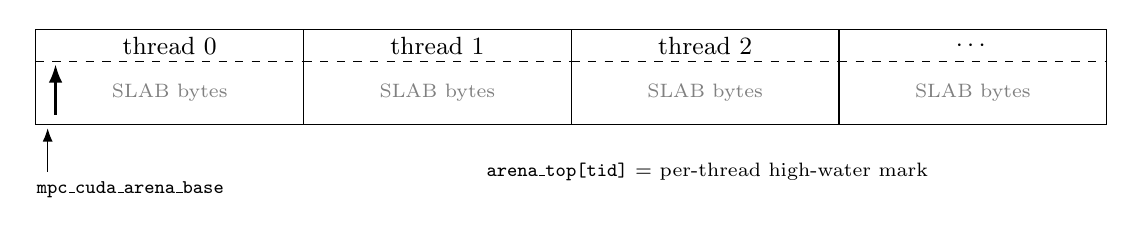
\begin{tikzpicture}[x=1mm,y=1mm,font=\small]
  \def\w{34}
  \foreach \i/\lab in {0/{thread 0},1/{thread 1},2/{thread 2},3/{$\cdots$}}{
    \draw (\i*\w,0) rectangle (\i*\w+\w,12);
    \draw[dashed] (\i*\w,8) -- (\i*\w+\w,8);
    \node at (\i*\w+\w/2,10) {\lab};
    \node[font=\scriptsize,gray] at (\i*\w+\w/2,4) {SLAB bytes};
  }
  % bump arrow inside slab 0 (allocations grow upward)
  \draw[-{Latex},thick] (2.5,1.2) -- (2.5,7.6);
  \draw[-{Latex}] (1.5,-6) -- (1.5,-0.5);
  \node[anchor=north,font=\scriptsize] at (12,-6) {\code{mpc\_cuda\_arena\_base}};
  \node[anchor=west,font=\scriptsize] at (\w+22,-6)
    {\code{arena\_top[tid]} $=$ per-thread high-water mark};
\end{tikzpicture}
\caption{The per-thread bump arena: one \code{cudaMalloc} block split into a
fixed-size slab per resident thread. Allocate bumps the thread's offset; free is a
no-op; reset zeroes it. No two threads share a slab, so there is no contention.}
\label{fig:arena}
\end{figure}

\paragraph{Sizing.}
Total arena memory is $\textsc{launch}\times\textsc{slab}$: \textsc{launch} the
fixed number of resident threads (chosen for occupancy---the deep call chains keep
limbs in global-memory slabs, so many warps are needed to hide that latency), and
\textsc{slab} the per-thread scratch, which must hold one work item's peak
simultaneously-live allocation. Because free is a no-op, that peak equals
everything allocated since the last reset, and it is directly measurable:
\code{mpc\_cuda\_arena\_top[tid]} \emph{is} the high-water mark, so running one
work item without resetting reports the exact byte count. Scratch scales roughly
linearly with precision; empirically (at 1024 bits) a real MPFR \code{axpy}/dot
needs $\approx 32$\,KB per thread and a complex MPC one $\approx 256$\,KB (about
$8\times$, complex chains being deeper). Over-provisioning only costs memory;
under-provisioning silently drops onto the slow path.

\subsection{Device-correct division}
\label{sec:div}

MPFR's generic division (\code{mpfr\_div}, the divide-and-conquer / short-division
path of \cite{HarveyZimmermann,MollerGranlund}) miscompiles under \code{nvcc} for
precisions of three limbs or more, returning \code{inf} or garbage on the device.
The fault was root-caused to the optimizer but the offending construct resisted
isolation, and lower-level building blocks (\code{mpn\_divrem}, mini-GMP \code{mpz}
division, \code{udiv\_qrnnd}, \code{count\_leading\_zeros}) are all
\emph{verified correct} on the device. \code{mpc\_cuda} therefore substitutes, on
the device only, a self-contained correctly-rounded division built solely on the
trusted \code{mpz} primitives; the host keeps upstream MPFR. Division is the
foundation of the constants and transcendentals (which divide internally), so this
substitution is what unblocks the whole runtime layer.

\begin{algorithm}[h]
\caption{\code{mpfr\_div\_cuda}$(u,v,\mathit{rnd})$: device-correct, correctly-rounded division}
\label{alg:div}
\begin{algorithmic}[1]
\Require finite nonzero $u,v$ of precision $\le$ that of the destination $q$ (\PB{} bits); singular cases ($0,\infty,\mathrm{NaN}$) handled separately as in MPFR.
\State $s \gets \operatorname{sign}(u)\cdot\operatorname{sign}(v)$
\State Build the significands of $u$ and $v$ as integers $M_u,M_v$ (\code{mpz})
\State $\mathit{shift} \gets \PB + 2 + (\text{limb count of }v)\cdot 64$ \Comment{guard bits for one exact quotient}
\State $\mathit{num} \gets M_u \ll \mathit{shift}$
\State $(Q,R) \gets \code{mpz\_tdiv\_qr}(\mathit{num},\,M_v)$ \Comment{one exact integer division}
\State derive the round bit and sticky bit ($\mathit{sticky}=[R\neq 0]$ ORed with dropped low bits of $Q$)
\State normalise $Q$ to \PB{} bits, set the quotient exponent from $e_u-e_v$ and the shift
\State apply the rounding mode $\mathit{rnd}$ to $(Q,\text{round},\text{sticky})$; set sign $s$
\State \Return \code{mpfr\_check\_range}$(q)$ \Comment{matches host \code{mpfr\_div} bit-for-bit}
\end{algorithmic}
\end{algorithm}

The quotient is formed by a single \code{mpz\_tdiv\_qr} of the numerator scaled by
$\PB+2$ guard bits (plus a full divisor's worth, so the integer quotient already
contains the target significand, a round bit, and enough material to decide
sticky). Rounding then follows MPFR exactly, for \emph{all} rounding modes, so
the public \code{cu\_mpfr\_div} is bit-identical to host \code{mpfr\_div}. The
cost is one big-integer division of $O(\PB)$ limbs; it is asymptotically the same
class as MPFR's path and is invisible to the caller.

\subsection{Functions that are host-only}
Formatted and string I/O (\code{mpfr\_printf}, \code{mpfr\_get\_str} parsing,
\code{mpfr\_set\_str}, \code{mpz\_out\_str}, \ldots) and the \code{mpf\_t}/\code{mpq\_t}
conversions absent from mini-GMP are not available on the device; their device
stubs trap if called. These are not algorithmic changes, only surface
restrictions, but they bound what a kernel may call.


\section{Fixed-precision real type \texorpdfstring{\code{cu\_freal<\PB>}}{cu\_freal<PB>}}
\label{sec:freal}

When the precision is known at compile time, \code{cu\_freal<\PB>} (header
\code{cu\_freal.cuh}) holds the whole number in registers and dispenses with the
arena and the runtime-precision dispatch. \PB{} is any positive multiple of $32$
(so $\mathit{SB}\in\{0,32\}$), and the significand occupies $\Nlimb=\lceil\PB/64\rceil$
limbs. Every operation is bit-exact with MPFR \rndn.

\subsection{Storage}
\label{sec:freal-storage}

A value is a triple \code{(sign, exp, m[N])} realising \eqref{eq:model}:
\code{sign}$\in\{\pm1\}$, \code{exp} the MPFR exponent, and \code{m} the
left-justified significand (Figure~\ref{fig:layout}). A reserved exponent flags
zero. Because the layout matches MPFR's, conversion to/from a runtime
\code{cu\_mpfr\_t} of the same precision is a copy.

\begin{figure}[h]
\centering
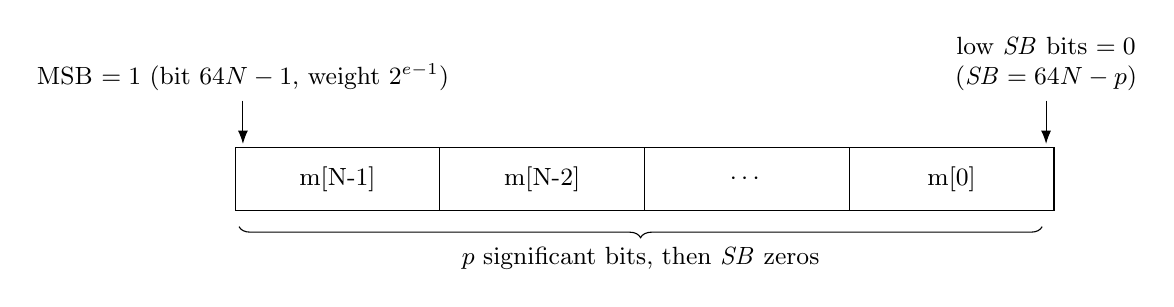
\begin{tikzpicture}[x=1mm,y=1mm,font=\small]
  % limb boxes m[N-1] ... m[0]
  \def\w{26}
  \foreach \i/\lab in {0/{m[N-1]},1/{m[N-2]},2/{$\cdots$},3/{m[0]}}{
    \draw (\i*\w,0) rectangle (\i*\w+\w,8);
    \node at (\i*\w+\w/2,4) {\lab};
  }
  % MSB marker
  \draw[-{Latex}] (1,14) -- (1,8.5);
  \node[anchor=south] at (1,14) {MSB $=1$ (bit $64N-1$, weight $2^{e-1}$)};
  % SB low zero bits
  \draw[-{Latex}] (3*\w+\w-1,14) -- (3*\w+\w-1,8.5);
  \node[anchor=south,align=center] at (3*\w+\w-1,14) {low $\mathit{SB}$ bits $=0$\\($\mathit{SB}=64N-\PB$)};
  % bracket for P significant bits
  \draw[decorate,decoration={brace,amplitude=4pt,mirror}] (0.5,-2) -- (3*\w+\w-1.5,-2)
    node[midway,below=4pt] {\PB{} significant bits, then $\mathit{SB}$ zeros};
\end{tikzpicture}
\caption{Left-justified significand of \code{cu\_freal<\PB>}: $\Nlimb$ limbs,
high to low, MSB always set, low $\mathit{SB}$ bits forced zero. Identical to
MPFR's in-memory layout.}
\label{fig:layout}
\end{figure}

\subsection{The rounding kernel \texttt{finalize}}
\label{sec:finalize}

All real operations funnel through one routine, \code{finalize}, which takes an
exact magnitude (a little-endian limb buffer $D$ with a known MSB position and
exponent, plus round/sticky material that lies \emph{below} $D$) and produces the
\rndn-rounded \code{cu\_freal<\PB>}. This single point of rounding is what makes
the type provably bit-exact with MPFR: every kernel below is responsible only for
forming an \emph{exact} intermediate and handing it to \code{finalize}.

\begin{figure}[h]
\centering
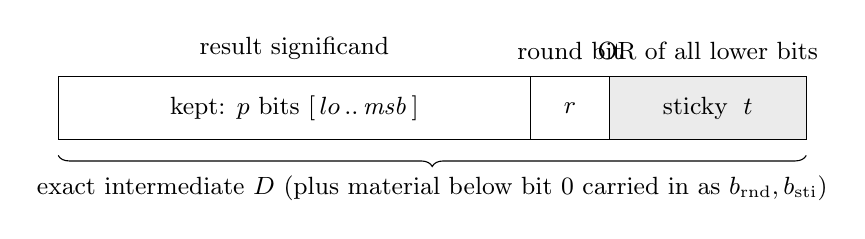
\begin{tikzpicture}[x=1mm,y=1mm,font=\small]
  \draw (0,0) rectangle (60,8); \node at (30,4) {kept: \PB{} bits $[\,lo\,..\,\mathit{msb}\,]$};
  \draw (60,0) rectangle (70,8); \node at (65,4) {$r$};
  \draw[fill=black!8] (70,0) rectangle (95,8); \node at (82.5,4) {sticky $\;t$};
  \node[anchor=south] at (30,9) {result significand};
  \node[anchor=south] at (65,9) {round bit};
  \node[anchor=south] at (82.5,9) {OR of all lower bits};
  \draw[decorate,decoration={brace,amplitude=4pt,mirror}] (0,-2) -- (95,-2)
    node[midway,below=4pt] {exact intermediate $D$ (plus material below bit $0$ carried in as $b_{\mathrm{rnd}},b_{\mathrm{sti}}$)};
\end{tikzpicture}
\caption{Decision bits used by \code{finalize}: the \PB{} kept bits, the round
bit $r$ immediately below them, and the sticky bit $t$ (logical OR of everything
still lower). Round-to-nearest-even increments iff $r\wedge(t\vee \text{lsb})$.}
\label{fig:round}
\end{figure}

\begin{algorithm}[h]
\caption{\code{finalize}$(D,\mathit{msb},E_{\mathrm{hi}},b_{\mathrm{rnd}},b_{\mathrm{sti}},s)$}
\label{alg:finalize}
\begin{algorithmic}[1]
\State $lo \gets \mathit{msb}-\PB+1$ \Comment{lowest kept bit position in $D$}
\If{$lo>0$}
  \State $V \gets$ bits $[\,lo\,..\,lo+\PB-1\,]$ of $D$;\quad $r \gets D_{lo-1}$;\quad $t \gets b_{\mathrm{rnd}}\vee b_{\mathrm{sti}}\vee \big(\textstyle\bigvee_{i<lo-1} D_i\big)$
\ElsIf{$lo=0$}
  \State $V \gets D$;\quad $r \gets b_{\mathrm{rnd}}$;\quad $t \gets b_{\mathrm{sti}}$
\Else
  \State $V \gets D \ll (-lo)$;\quad $r \gets 0$;\quad $t \gets 0$ \Comment{$<\PB$ significant bits: exact}
\EndIf
\If{$r \wedge (t \vee (V \bmod 2))$} \Comment{round to nearest, ties to even}
  \State $V \gets V+1$
  \If{$V$ carried out of bit $\PB-1$} \State $V \gets 2^{\PB-1}$;\quad $E_{\mathrm{hi}} \gets E_{\mathrm{hi}}+1$ \EndIf
\EndIf
\State $m \gets V \ll \mathit{SB}$;\quad $\code{exp} \gets E_{\mathrm{hi}}+1$;\quad $\code{sign}\gets s$
\State \Return \code{(sign, exp, m)}
\end{algorithmic}
\end{algorithm}

The three branches handle the normal case, the aligned case, and the
fewer-than-\PB-bit (hence exact) case; the carry-out branch handles the
$1.\overline{1}\!\to\!10.0$ overflow by bumping the exponent. Conversions from
\code{double} (\code{from\_double}) and to \code{double} (\code{to\_double}) use
the same round-bit/sticky-bit logic on the 53-bit IEEE mantissa.

\subsection{Multiplication}
\label{sec:freal-mul}

Multiplication forms the \emph{exact} $2\Nlimb$-limb product with a
register-resident schoolbook $O(\Nlimb^2)$ multiply
(Figure~\ref{fig:mul}), then normalises and rounds it through \code{finalize}.
Because \PB{} is a compile-time constant the double loop is fully unrolled and
\code{ptxas} keeps every limb in a register; on the device each $64\times64\to128$
step is a \code{mad.lo.cc.u64}/\code{madc.hi.u64} pair, so the inner product runs
with no global-memory traffic.

\begin{figure}[h]
\centering
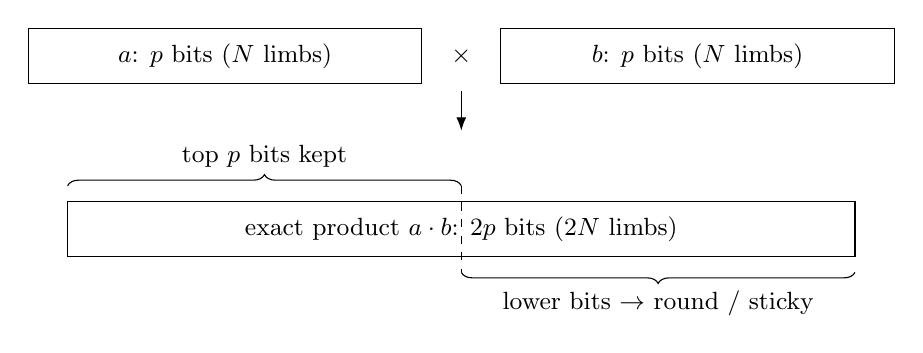
\begin{tikzpicture}[x=1mm,y=1mm,font=\small]
  \draw (0,0) rectangle (50,7); \node at (25,3.5) {$a$: \PB{} bits ($\Nlimb$ limbs)};
  \draw (60,0) rectangle (110,7); \node at (85,3.5) {$b$: \PB{} bits ($\Nlimb$ limbs)};
  \node at (55,3.5) {$\times$};
  \draw[-{Latex}] (55,-1) -- (55,-6);
  \draw (5,-22) rectangle (105,-15);
  \node at (55,-18.5) {exact product $a\cdot b$: $2\PB$ bits ($2\Nlimb$ limbs)};
  % cut line for kept P bits
  \draw[dashed] (55,-13) -- (55,-24);
  \draw[decorate,decoration={brace,amplitude=4pt}] (5,-13) -- (55,-13)
     node[midway,above=3pt] {top \PB{} bits kept};
  \draw[decorate,decoration={brace,amplitude=4pt,mirror}] (55,-24) -- (105,-24)
     node[midway,below=3pt] {lower bits $\to$ round / sticky};
\end{tikzpicture}
\caption{Fixed-precision multiply: the exact $2\PB$-bit product is computed in
registers, then its top \PB{} bits are kept and the remainder feeds the
round/sticky decision of \code{finalize}. The result equals
$\round(a\cdot b)$, i.e.\ \code{mpfr\_mul} at \PB{} bits.}
\label{fig:mul}
\end{figure}

\subsection{Addition and subtraction}
\label{sec:freal-add}

Addition aligns the smaller operand by the exponent difference $d=e_a-e_b$,
capturing the bits shifted past limb $0$ as round/sticky, sums into an
$\Nlimb{+}1$-limb buffer, and rounds (Figure~\ref{fig:add}). Subtraction of like
signs uses a buffer with two guard limbs (128 extra bits) so that catastrophic
cancellation still leaves a correctly-rounded result: the exact difference is
formed, the leading nonzero bit located, and \code{finalize} rounds from there.
Same-sign/opposite-sign dispatch and the magnitude comparison mirror MPFR's
\code{mpfr\_add}/\code{mpfr\_sub}.

\begin{figure}[h]
\centering
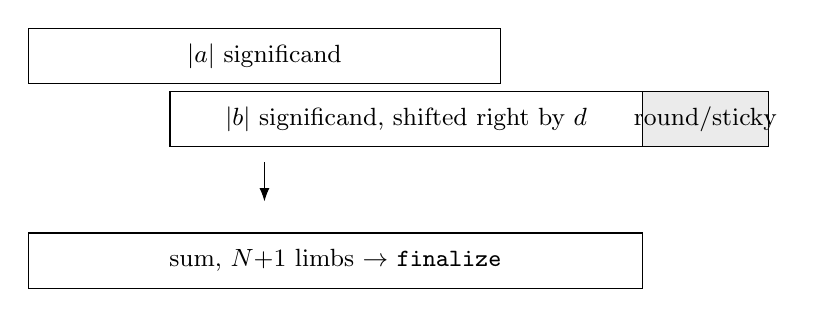
\begin{tikzpicture}[x=1mm,y=1mm,font=\small]
  \draw (0,8) rectangle (60,15); \node at (30,11.5) {$|a|$ significand};
  \draw (18,0) rectangle (78,7);  \node at (48,3.5) {$|b|$ significand, shifted right by $d$};
  \draw[fill=black!8] (78,0) rectangle (94,7); \node at (86,3.5) {round/sticky};
  \draw[-{Latex}] (30,-2) -- (30,-7);
  \draw (0,-18) rectangle (78,-11); \node at (39,-14.5) {sum, $\Nlimb{+}1$ limbs $\to$ \code{finalize}};
\end{tikzpicture}
\caption{Fixed-precision add: align $|b|$ by $d=e_a-e_b$, keep the shifted-out
bits as round/sticky, add, then round once. Subtraction uses two extra guard
limbs to absorb cancellation.}
\label{fig:add}
\end{figure}

\subsection{Cost}
With $\Nlimb=\lceil\PB/64\rceil$, multiplication is $O(\Nlimb^2)$ word
multiplies and add/sub are $O(\Nlimb)$, all register-resident with no allocation.
The schoolbook multiply is asymptotically inferior to GMP/MPFR's
sub-quadratic multiplication, so the fixed-precision advantage is greatest at
low and medium precision (where keeping limbs in registers dominates) and erodes
once the working set spills out of registers at high \PB.


\section{Fixed-precision complex type \texorpdfstring{\code{cu\_fcomplex<\PB>}}{cu\_fcomplex<PB>}}
\label{sec:fcomplex}

\code{cu\_fcomplex<\PB>} (header \code{cu\_fcomplex.cuh}) is a pair of
\code{cu\_freal<\PB>} components. Addition and subtraction are componentwise
\code{cu\_fadd}/\code{cu\_fsub}, hence trivially \code{MPC\_RNDNN}. The
interesting operation is multiplication, which is made \emph{correctly rounded per
component}---bit-exact with MPC's \code{MPC\_RNDNN}---by avoiding double rounding.

\subsection{Exact fused \texorpdfstring{$\fmms$/$\fmma$}{fmms/fmma}}
\label{sec:fmms}

The naive complex product $\Re = ar\,br - ai\,bi$, $\Im = ar\,bi + ai\,br$ rounds
each of the four real products before subtracting/adding, incurring two
roundings per component and so failing to match MPC. Instead \code{mpc\_cuda}
evaluates each component with a single rounding via the fused primitives
\begin{align}
\fmms(a,b,c,d) &= \round(a\,b - c\,d), &
\fmma(a,b,c,d) &= \round(a\,b + c\,d),
\end{align}
each computed from the two \emph{exact} $2\Nlimb$-limb products combined with a
\emph{single} \rndn{} rounding (Figure~\ref{fig:fmms}). Concretely each product
$a\,b$ and $c\,d$ is formed exactly by the schoolbook multiply of
\S\ref{sec:freal-mul} and normalised to a signed wide term
$\code{(sign},\code{exp},M[2\Nlimb])$; the two wide terms are then aligned by
their exponent difference (with three guard limbs), added or subtracted exactly,
and rounded once by \code{finalize}. The result therefore equals
$\round(ab\pm cd)$ with no intermediate rounding, which is precisely what MPFR's
\code{mpfr\_fmms}/\code{mpfr\_fmma} (and hence MPC) compute.

\begin{figure}[h]
\centering
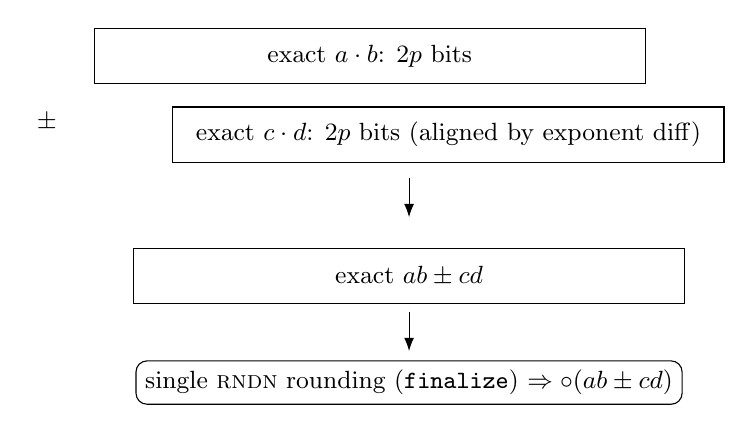
\begin{tikzpicture}[x=1mm,y=1mm,font=\small]
  \draw (0,16) rectangle (70,23);  \node at (35,19.5) {exact $a\cdot b$: $2\PB$ bits};
  \draw (10,6) rectangle (80,13);  \node at (45,9.5) {exact $c\cdot d$: $2\PB$ bits (aligned by exponent diff)};
  \node at (-6,11) {$\pm$};
  \draw[-{Latex}] (40,4) -- (40,-1);
  \draw (5,-12) rectangle (75,-5); \node at (40,-8.5) {exact $ab\pm cd$};
  \draw[-{Latex}] (40,-13) -- (40,-18);
  \node[draw,rounded corners] at (40,-22) {single \rndn{} rounding (\code{finalize}) $\Rightarrow \round(ab\pm cd)$};
\end{tikzpicture}
\caption{Exact fused $\fmms/\fmma$: both $2\PB$-bit products are kept exact,
aligned, combined, and rounded \emph{once}. No double rounding, so each component
matches MPC's \code{MPC\_RNDNN} bit-for-bit.}
\label{fig:fmms}
\end{figure}

\subsection{Complex multiply}
With the fused primitives, complex multiplication is the textbook identity
evaluated component-exact:
\begin{equation}
(ar+i\,ai)(br+i\,bi) \;=\; \underbrace{\fmms(ar,br,ai,bi)}_{\Re=\round(ar\,br-ai\,bi)}
\;+\; i\,\underbrace{\fmma(ar,bi,ai,br)}_{\Im=\round(ar\,bi+ai\,br)} .
\end{equation}
This is the ``$3M$-free'', accuracy-first formulation: four exact products, two
single-rounded combinations, validated bit-exact against MPC over $\PB=32\ldots
2048$.


\section{Fixed-precision elementary functions}
\label{sec:elem}

The elementary functions (headers \code{cu\_fmath.cuh} for real,
\code{cu\_fcmath.cuh} for complex) trade correct rounding for register residency.
Each function evaluates at a \emph{working precision}
\begin{equation}
W \;=\; \PB + g, \qquad g = \texttt{CU\_FGUARD} = 128~\text{bits (default)},
\end{equation}
using Newton iteration and argument-reduced series in \code{cu\_freal<$W$>}, then
re-rounds the $W$-bit result back to \PB. Results are \emph{faithful} to about
\PB{} bits and agree with MPFR/MPC to $\lesssim 1\,\ulp$ in the common range.
They are deliberately \emph{not} correctly rounded: the table-maker's dilemma
would require an unbounded Ziv loop, incompatible with a fixed register budget.
Use the runtime \code{cu\_mpfr}/\code{cu\_mpc} API when last-bit correctness is
required.

\subsection{Newton kernels (division, square root, cube root)}
Each algebraic function iterates a self-correcting Newton map seeded from the
\code{double} approximation; the number of iterations is
$\lceil\log_2(W/52)\rceil+1$, doubling the correct digits each step
(Table~\ref{tab:newton}).

\begin{table}[h]
\centering
\begin{tabular}{@{}llll@{}}
\toprule
Function & Quantity & Newton update & Reconstruction\\
\midrule
\code{cu\_fdiv}  & reciprocal $z\!\approx\!1/m$ & $z \leftarrow z\,(2 - m z)$ & $a/b = a\cdot(1/b)$\\
\code{cu\_sqrt}  & rsqrt $y\!\approx\!1/\sqrt m$ & $y \leftarrow \tfrac{1}{2}\,y\,(3 - m y^2)$ & $\sqrt m = m\cdot y$\\
\code{cu\_cbrt}  & rcbrt $y\!\approx\!m^{-1/3}$ & $y \leftarrow y\,(4 - m y^3)/3$ & $\sqrt[3]{m}=m\,y^2$\\
\bottomrule
\end{tabular}
\caption{Division-free Newton iterations used by the fixed-precision algebraic
functions. $m$ is the mantissa after binary scaling into a fixed range; the power
of two is reattached afterward.}
\label{tab:newton}
\end{table}

The reciprocal iteration uses only multiplies and a subtract (no division), which
is why even \code{cu\_fdiv} avoids a hardware divide; \code{cu\_div\_ui} (division
by a small $<2^{32}$ integer) is a separate, correctly-rounded limb-by-limb
routine used inside the series.

\subsection{Transcendental functions: range reduction then series}
The transcendentals reduce the argument into a small interval, sum a Taylor (or
\code{atanh}/\code{atan}) series until the term drops below the working-precision
threshold, and reconstruct. The schemes are summarised in
Table~\ref{tab:trans}; constants $\ln 2$ and $\pi$ are themselves computed at
working precision by $2\,\operatorname{atanh}(1/3)$ and Machin's
$16\arctan(1/5)-4\arctan(1/239)$.

\begin{table}[h]
\centering
\renewcommand{\arraystretch}{1.2}
\begin{tabular}{@{}lp{0.46\linewidth}p{0.30\linewidth}@{}}
\toprule
Function & Reduction & Series / reconstruction\\
\midrule
\code{cu\_exp} & $x = k\ln 2 + r$, $k=\lfloor x/\ln2\rceil$; halve $r\!\to\!r/2^{m}$ until $|r|$ small & $\exp(r)=\sum r^n/n!$, square $m$ times, scale by $2^{k}$\\
\code{cu\_log} & $x=2^{e}m$, $m\in[\tfrac{1}{\sqrt2},\sqrt2)$;\ $t=\frac{m-1}{m+1}$ & $\log m = 2\operatorname{atanh}(t)$, add $e\ln2$\\
\code{cu\_sin/cos} & $x=k\frac{\pi}{2}+r$, $|r|\le\frac{\pi}{4}$; halve $r$ & Taylor for $\sin r,\cos r$, double-angle back, quadrant select on $k\bmod4$\\
\code{cu\_atan} & reduce to $|x|\le1$ via $1/x$; $a\leftarrow a/(1+\sqrt{1+a^2})$ & $\arctan$ series, scale by $2^{\text{(\#reductions)}}$\\
\code{cu\_asin/acos} & $\arcsin x=\arctan\!\big(x/\sqrt{1-x^2}\big)$; $\arccos = \pi/2-\arcsin$ & via \code{cu\_atan}\\
\code{cu\_sinh/cosh} & via $e^{x}$ (small-$x$ Taylor for $\sinh$) & $\tfrac12(e^x\mp e^{-x})$\\
\code{cu\_atanh} & $|x|\le\tfrac12$ series; else $\tfrac12\log\frac{1+x}{1-x}$ & \code{atanh} series / \code{cu\_log}\\
\code{cu\_pow} & $x^y=\exp(y\log x)$ ($x>0$); integer-$y$ branch for $x<0$ & via \code{cu\_exp}, \code{cu\_log}\\
\bottomrule
\end{tabular}
\caption{Argument reduction and reconstruction for the fixed-precision
transcendentals. All intermediates are \code{cu\_freal<$W$>} with $W=\PB+128$.}
\label{tab:trans}
\end{table}

\subsection{Complex elementary functions}
The complex layer (\code{cu\_fcmath.cuh}: \code{cu\_cexp}, \code{cu\_clog},
\code{cu\_csqrt}, \code{cu\_csin}, \code{cu\_ccos}, \code{cu\_ctan},
\code{cu\_csinh}, \code{cu\_ccosh}, \code{cu\_cdiv}, and \code{atan2}) is built
from the real functions plus the \emph{exact} $\fmms/\fmma$ of
\S\ref{sec:fmms} for every squared-modulus and cross term, e.g.
\begin{align}
|z|^2 &= \fmma(\Re z,\Re z,\Im z,\Im z), &
\log z &= \tfrac12\log|z|^2 + i\,\operatorname{atan2}(\Im z,\Re z),\\
e^{z} &= e^{\Re z}\,(\cos\Im z + i\sin\Im z), &
\tfrac{a}{b} &= \frac{\fmma(ar,br,ai,bi) + i\,\fmms(ai,br,ar,bi)}{\fmma(br,br,bi,bi)} .
\end{align}
Using the exact fused products for $|b|^2$ and the numerators keeps the complex
divide and the modulus from losing accuracy to double rounding. Like their real
counterparts these are faithful, $\lesssim 1\,\ulp$ vs MPC.


\section{Accuracy and validation}
\label{sec:accuracy}

\begin{table}[h]
\centering
\begin{tabular}{@{}p{0.34\linewidth}p{0.30\linewidth}p{0.28\linewidth}@{}}
\toprule
Operation & Guarantee & Validation range\\
\midrule
runtime \code{cu\_mpfr}/\code{cu\_mpc} (incl.\ \code{cu\_mpfr\_div}) & correctly rounded, all modes; bit-identical to host & matches host MPFR/MPC\\
\code{cu\_freal} $+,-,\times$ & bit-exact MPFR \rndn & $\PB=32\ldots2048$\\
\code{cu\_fcomplex} $+,-,\times$ & bit-exact \code{MPC\_RNDNN} & $\PB=32\ldots2048$\\
\code{cu\_fmath}/\code{cu\_fcmath} & faithful, $\lesssim 1\,\ulp$ (not correctly rounded) & $\PB=64\ldots1024$\\
\bottomrule
\end{tabular}
\caption{Accuracy contract per operation and the validated precision ranges.}
\label{tab:accuracy}
\end{table}

The two basic-arithmetic claims are checked bit-for-bit against the system MPFR
and MPC; the elementary-function claim is checked in \ulp{} against MPFR/MPC (the
shipped suite reports $0\,\ulp$ in its sampled inputs, with $\le 1\,\ulp$ the
designed bound). The contracts are summarised in Table~\ref{tab:accuracy}.


\section{How to cite}
\label{sec:cite}

This document describes the algorithms of \code{mpc\_cuda}. The two results most
likely to be cited are (i) the register-resident fixed-precision arithmetic that
is bit-exact with MPFR \rndn{} and MPC \code{MPC\_RNDNN} via a single rounding
point and exact fused $\fmms/\fmma$ (\S\ref{sec:freal}--\ref{sec:fcomplex}), and
(ii) the \code{mpz}-based correctly-rounded division that replaces MPFR's
generic path on the device (\S\ref{sec:div}). The companion technical report
(\code{mpc\_cuda\_report}) gives the performance evaluation, including the
GPU/CPU crossover and the $\sim\!140\times$ speedup of \code{cu\_freal} over the
runtime GPU path at 1024 bits for AXPY. The runtime layer's correctly-rounded
semantics follow MPFR \cite{MPFR} and MPC \cite{MPC}, themselves built on GMP
\cite{GMP}; the underlying methods are standard \cite{BrentZimmermann,Muller}.

\begin{thebibliography}{9}
\bibitem{GMP} T.~Granlund and the GMP development team,
  \emph{GNU MP: The GNU Multiple Precision Arithmetic Library}.
  \url{https://gmplib.org/}.
\bibitem{MPFR} L.~Fousse, G.~Hanrot, V.~Lef\`evre, P.~P\'elissier, P.~Zimmermann,
  ``MPFR: A multiple-precision binary floating-point library with correct
  rounding,'' \emph{ACM Trans.\ Math.\ Softw.}, 33(2), 2007.
  \url{https://www.mpfr.org/}.
\bibitem{MPC} A.~Enge, M.~Gastineau, P.~Th\'eveny, P.~Zimmermann,
  \emph{GNU MPC: A library for multiprecision complex arithmetic with exact
  rounding}. \url{https://www.multiprecision.org/mpc/}.
\bibitem{HarveyZimmermann} D.~Harvey and P.~Zimmermann,
  ``Short Division of Long Integers,''
  \emph{Proc.\ 20th IEEE Symp.\ on Computer Arithmetic (ARITH-20)}, 2011,
  pp.~7--14.
\bibitem{MollerGranlund} N.~M\"oller and T.~Granlund,
  ``Improved Division by Invariant Integers,''
  \emph{IEEE Trans.\ Computers}, 60(2):165--175, 2011.
\bibitem{BrentZimmermann} R.~P.~Brent and P.~Zimmermann,
  \emph{Modern Computer Arithmetic}, Cambridge University Press, 2010.
\bibitem{Muller} J.-M.~Muller et al.,
  \emph{Handbook of Floating-Point Arithmetic}, 2nd ed., Birkh\"auser, 2018.
\end{thebibliography}

\end{document}
